\documentclass[]{article}
\usepackage{fontspec}
\usepackage{graphicx}
\usepackage{float}
\usepackage[left=1.27cm,top=1.27cm,right=1.27cm,bottom=1.27cm]{geometry}
\usepackage{pbox}
\setmainfont{Cambria}

% If you use Biber, then you will have to compile and recompile.
% But Biber seems to be the preferred choice.
\usepackage[sorting=none,style=numeric-comp]{biblatex} 

\addbibresource{tmle} 

\begin{document}
\title{Hospital readmissions and targeted maximum likelihood estimation}
\author{Aman Verma}
\date{\today}
% \maketitle


\section{Introduction}
% Why is this question important to answer?
It is particularly important to accurately estimate the independent effect of hospital treatment on readmission because it is being used to financially penalize hospitals.

% Why it doesn't matter what a preventable readmission is if you have properly stated the counterfactual.

% What is the clear study question?
% How does this relate to the counterfactual statement?
What is the difference in the proportion with an emergency readmission within 30 days if all patients had attended Hospital A vs Hospital B? 

The notion of a "preventable" readmission is implicit; if a patient would have been readmitted if treated at another hospital, then the readmission was preventable. 

\section{Methods}

\subsection{Data}
% What does our cohort look like?

\subsubsection{Cohort selection}
We used a cohort extracted from a Canadian provincial (Quebec) administrative database of hospitalizations, obtained from the \emph{Régie de l'assurance maladie du Québec} (RAMQ). We enrolled patients into this cohort on the month that two conditions were satisfied: 1) they had at least one diagnosis of a respiratory illness (the exact list of respiratory International Classification of Diseases, 9th Revision [ICD-9] codes is given in the Appendix) between January 1st, 1996 and March 31, 2006 (the study period), while living in the 2006 census metropolitan area of Montreal, and 2) were at least 65 years of age. We used this cohort because it represents the majority of 65-year olds who were hospitalized in the region during the study period. 

From among this cohort, we selected hospital discharges for those who had accrued at least one year in the cohort at the time of admission. We restricted our data to only the discharges from the twenty hospitals with the most discharges of patients 65 years or older within the study period; the twenty hospitals accounted for 75\% of all such discharges.  We only selected hospital discharges which resulted from hospital stays of at least one day. Therefore, the earliest possible hospital discharge was January 2, 1997.

\subsubsection{Disease types}
From among the identified hospital discharges, we selected only those with one of three high-volume admission diagnoses with high rates of hospital readmissions: pneumonia, acute myocardial infarction (AMI), and heart failure, the three initial conditions selected by the Centers for Medicare and Medicaid Services (CMS) to implement the Hospital Readmissions Reduction Program mandated by the Affordable Care Act. We identified each of the admission diagnoses using ICD-9 codes; for pneumonia we used codes ranging from 480-487, for heart failure we used all 428 codes, and for AMI we used all 410 codes. The following methods were applied individually to all three disease subsets. 

\subsubsection{Hospital readmissions}
The unit of analysis in all models was the hospital discharge; a single patient could be discharged multiple times. A hospital readmission was defined as an emergency hospital admission to any Quebec hospital in the 30 days following a discharge.  A person who died or had a non-emergency readmission in the 30 days following discharge was considered not readmitted.
% Should I talk about the anonymization of hospitals?

% We had confounders.
\subsection{Confounders}
For each hospital discharge, we colllected variables that measured events that occurred prior to the hospital admission and which may confound the relationship between hospital care and readmission. We used the demographic characteristics (age at time of admission (years), sex, birth year-month), the number of previous readmissions (within the study period), the admission diagnosis (as measured by the specific ICD-9 code). We also included the day of week of discharge, which has been previously shown to have an association with readmissions, and the month of discharge, because we hypothesized that readmission risk would vary by seasons in Montreal.

Additionally, for each discharge, we collected the hospital diagnoses, hospital procedures, and drugs dispensed outside of the hospital recorded in the year preceding the admissionin in Quebec. The procedures performed were recorded in the Canadian Classification of Diagnostic, Therapeutic, and Surgical Procedures (CCP) system. Hospital diagnostic codes were coded using the ICD-9 system. Finally, drugs which were prescribed and dispensed outside the hospital, and were being taken on the day of admission were also recorded for each patient in the code commune system, which records chemical compound being taken. To ease computation, before fitting any model, we removed any diagnosis, procedure or drug that occurred less than 30 times among all discharges. We chose 30 because it appeared to be a natural breakpoint; if the number of variables included is a function \emph{f} of the threshold, then the first derivative of \emph{f} dropped at 30 for all three disease categories.

% What about the census tract of residence?

\subsection{Descriptive analysis}
% We plotted a choropleth of the rate of attendance at certain hospitals. We used the Canadian census ... actually the most meaningful baseline would be the number of person-years accrued in each census tract by all members of the cohort.

\subsection{Models}
\subsubsection{Model G - probability of exposure}
% We built a model G
We developed a multinomial model g that predicted the probability of exposure (admission to a particular one of twenty hospitals). 
% We used a random forest. It was a stump model. We calibrated it based on the weights of the hospital. It was multinomial in that we predicted 20 hospitals. We used 1200 trees. We measured the accuracy as a function of the number of grown trees. When measuring the accuracy, we only used "out-of-bag" discharges. We measured the calibration, similarly only using out-of-bag discharges. We investigated the top 10 variables most important variables, as measured by the Gini coefficient. Random forest traditionally gives classifies by vote; we converted this into a probability by taking the proportion of votes for each hospital (out-of-bag).

% Why did we choose random forest?

\subsubsection{Model Q - probability of outcome}
% We built a model Q
% We built another random forest model, very similar to the model for G, except that instead of predicting the choice of hospital, we predicted 30-day readmission. We also included a set of 19 indicator variables (or was it twenty?) for the hospital. This was also calibrated based on the inverse of the proportion of those readmitted.

% We also built fit a regularized logistic regression model for Q. We penalized the 

\subsubsection{Variable importance}
% What is the ref for the Gini coefficient?
For each tree, we calculated the out-of-bag decrease in Gini impurity when comparing the split nodes of the tree to the root. 
The Gini impurity at any node is, for all out-of-bag discharges.

% To calculate the Gini impurity..
For each hospital, the proportion of patients that chose this hospital $p_h$, multiplied by the probability of guessing that this patient would choose this hospital based on the distribution of patients $1-p_h$. Summed over all hospitals, this is the Gini impurity. Gini impurity is 1 when all patients chose the same hospital.

To assess the importance of the variables in predicting which hospital a patient will choose, for each tree, we calculate the decrease in Gini impurity between the root of the tree and the leaves. If the patients within the leaves of the tree made relatively homogeneous hospital choices, this variable predicts hospital choice well, and the Gini impurity will decrease.
 
To calculate the Gini variable importance criterion, we summed the Gini impurity decrease over all trees.


\subsubsection{Model Q* - updated targeted maximum likelihood estimation}

% We updated for Q*



% How does the fastimp function rank the importance of variables?
\subsection{Software}
We implemented the random forest using the "bigrf" \cite{lim_bigrf_2014} package . We implemented the GLM fitting using coordinate descent using the "glmnet" package \cite{friedman_regularization_2010}. We plotted our figures using the "ggplot2" package \cite{wickham_ggplot2_2009}.


\section{Results}
% A pretty map for pretty much no reason. It shows that indeed, certain hospitals attract the residents around them, and that this does not vary by disease.
\begin{figure}[H]
    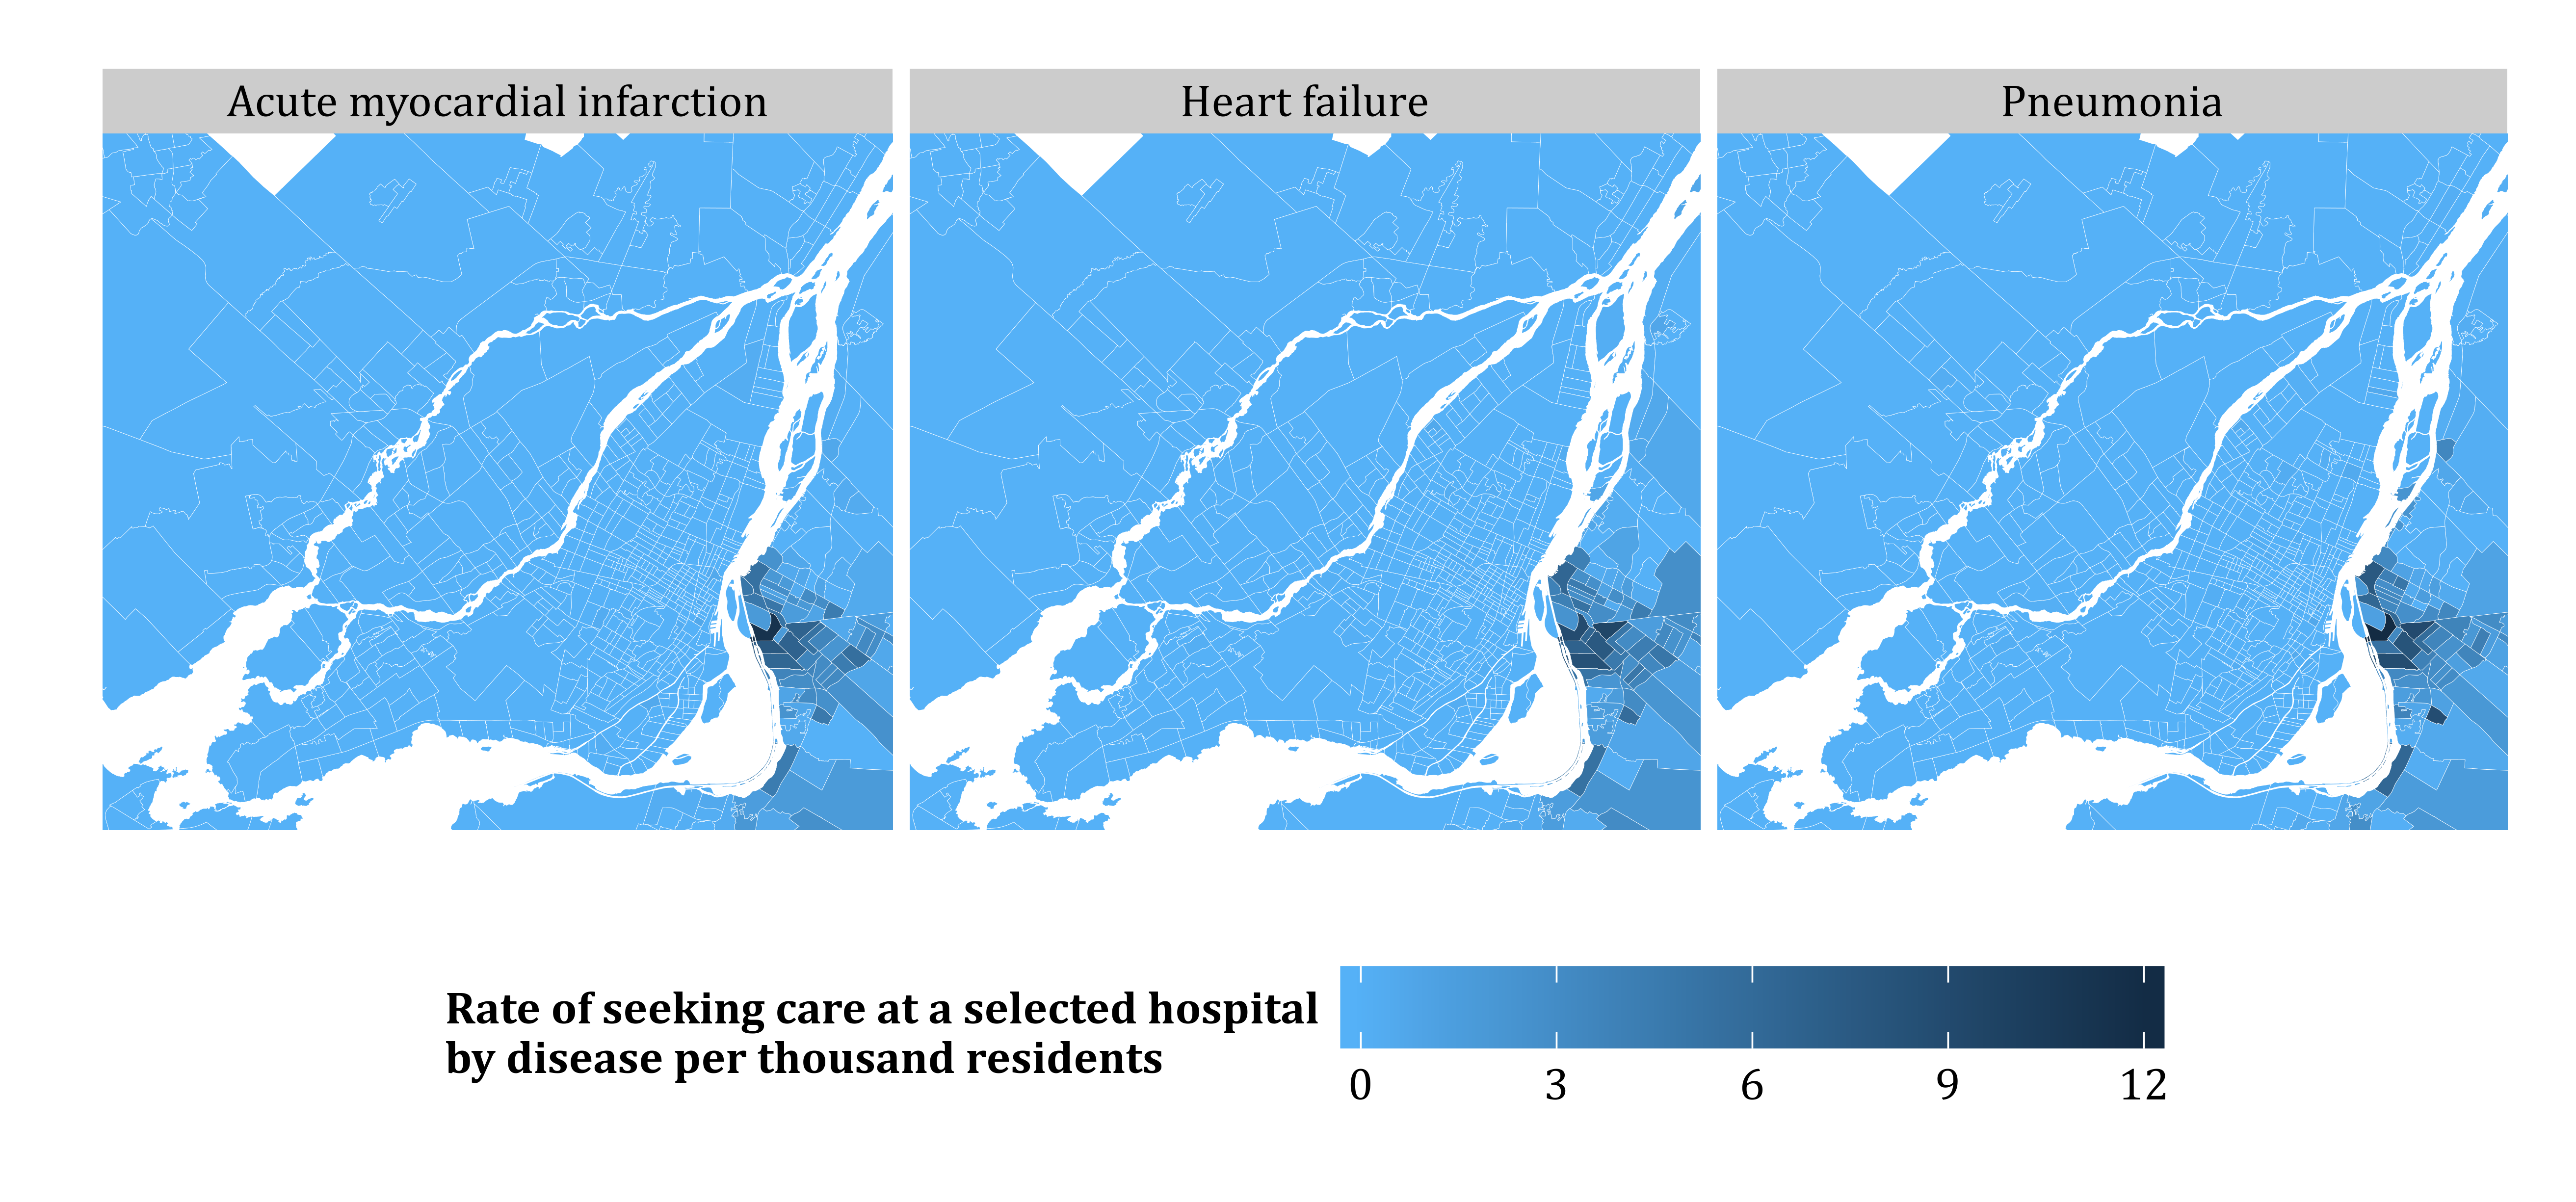
\includegraphics{../figures/hosp_choro.png}
    \caption[Rates of seeking care at a selected hospital by admission diagnosis.]
      {Rates of seeking care at a selected hospital by admission diagnosis. A descriptive sentence}
    \label{fig:hosp_choro}
\end{figure}

% What does the accuracy of the random forest model look like as the number of trees grows for both the Q model and the G model?
\begin{figure}[H]
    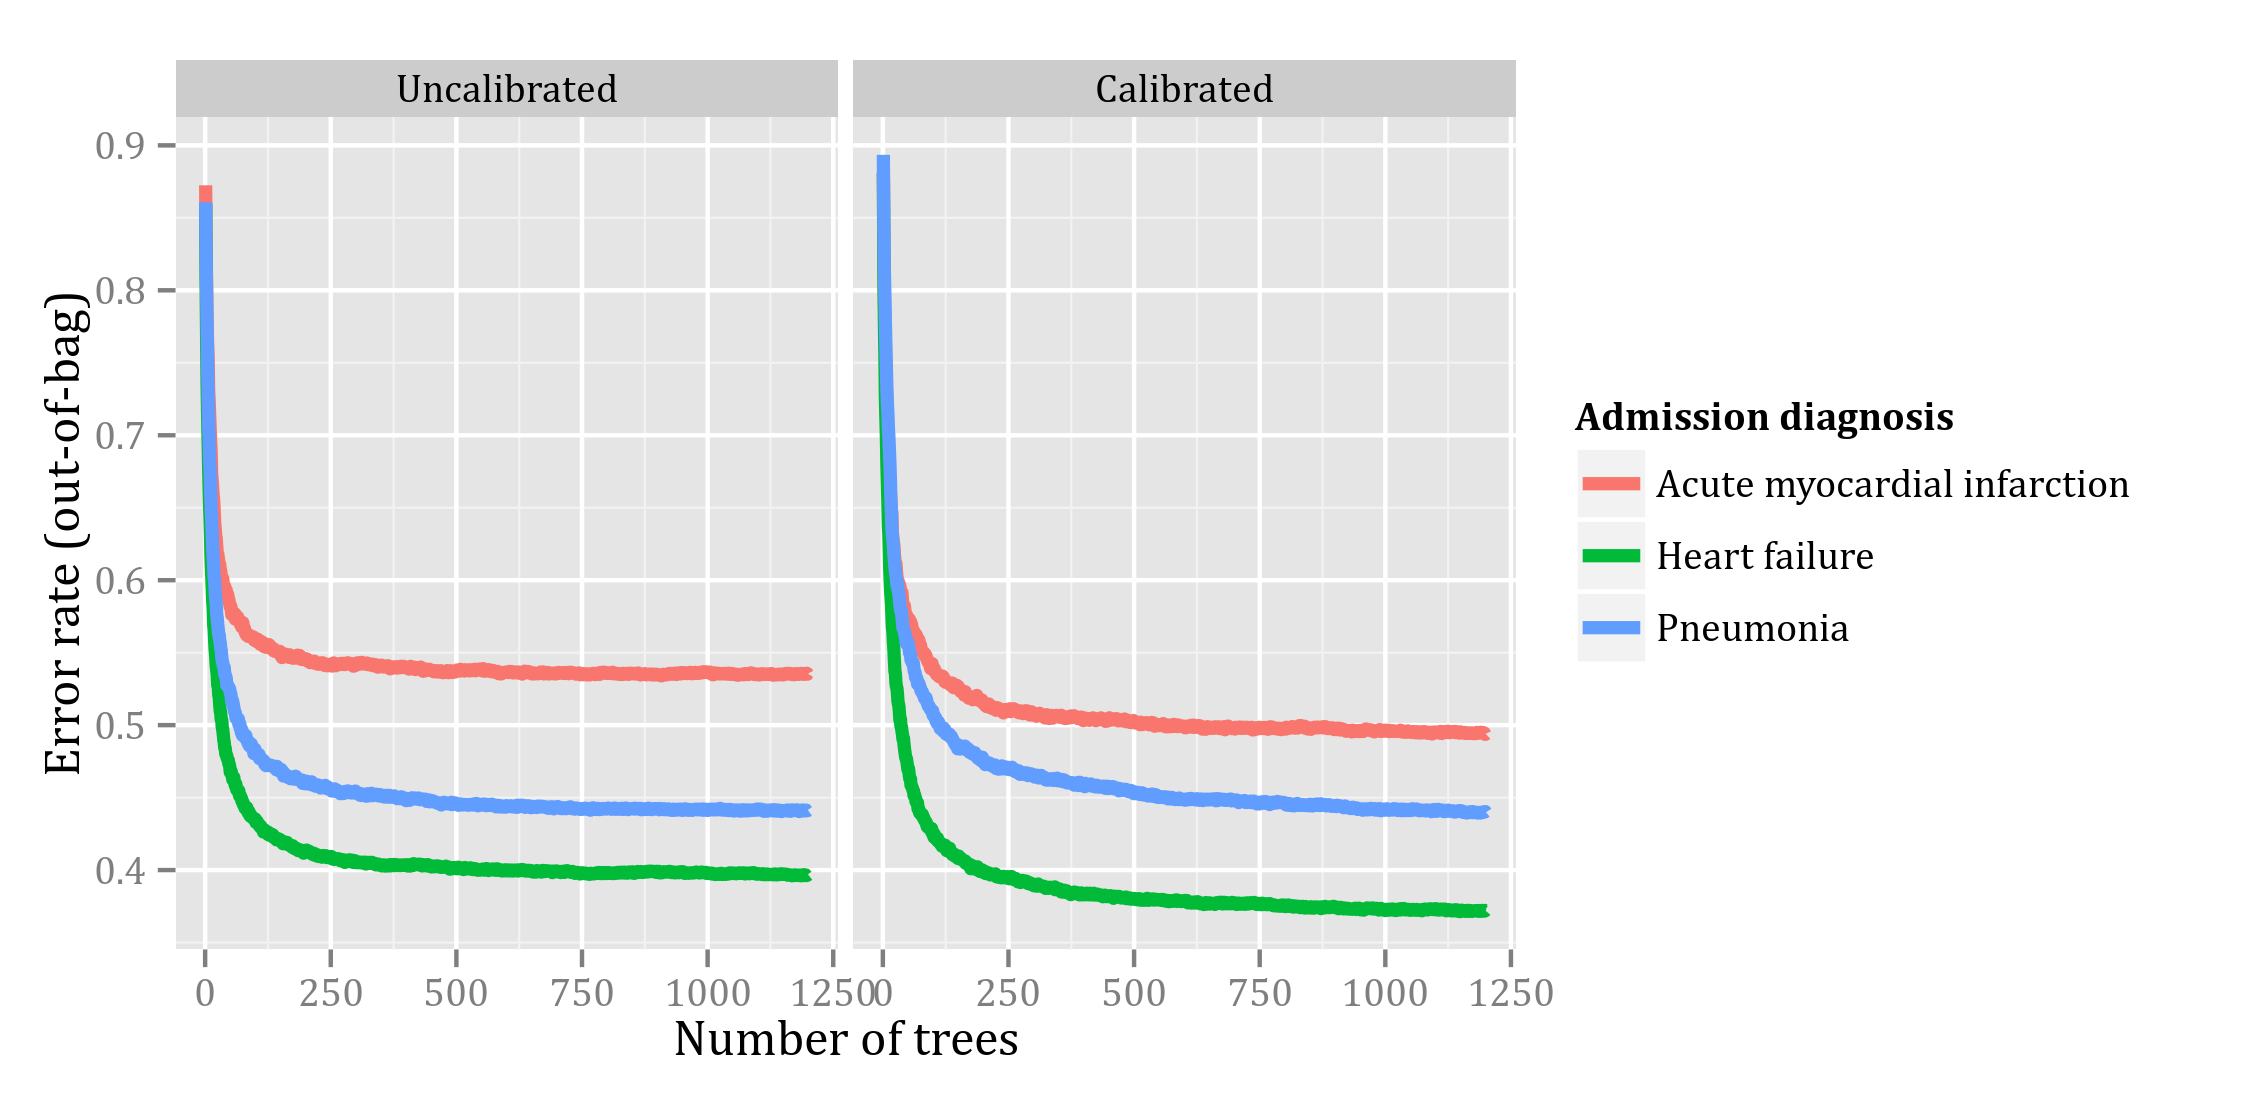
\includegraphics{../figures/error_rate_for_hospital_choice.png}
    \caption[Error rate for random forest model of hospital choice.]
      {Error rate for random forest model of hospital choice. A descriptive sentence.}
    \label{fig:error_rate_for_hospital_choice}
\end{figure}

% What are the top 10 predictive variables for the hospitals by disease?
\begin{figure}[H]
    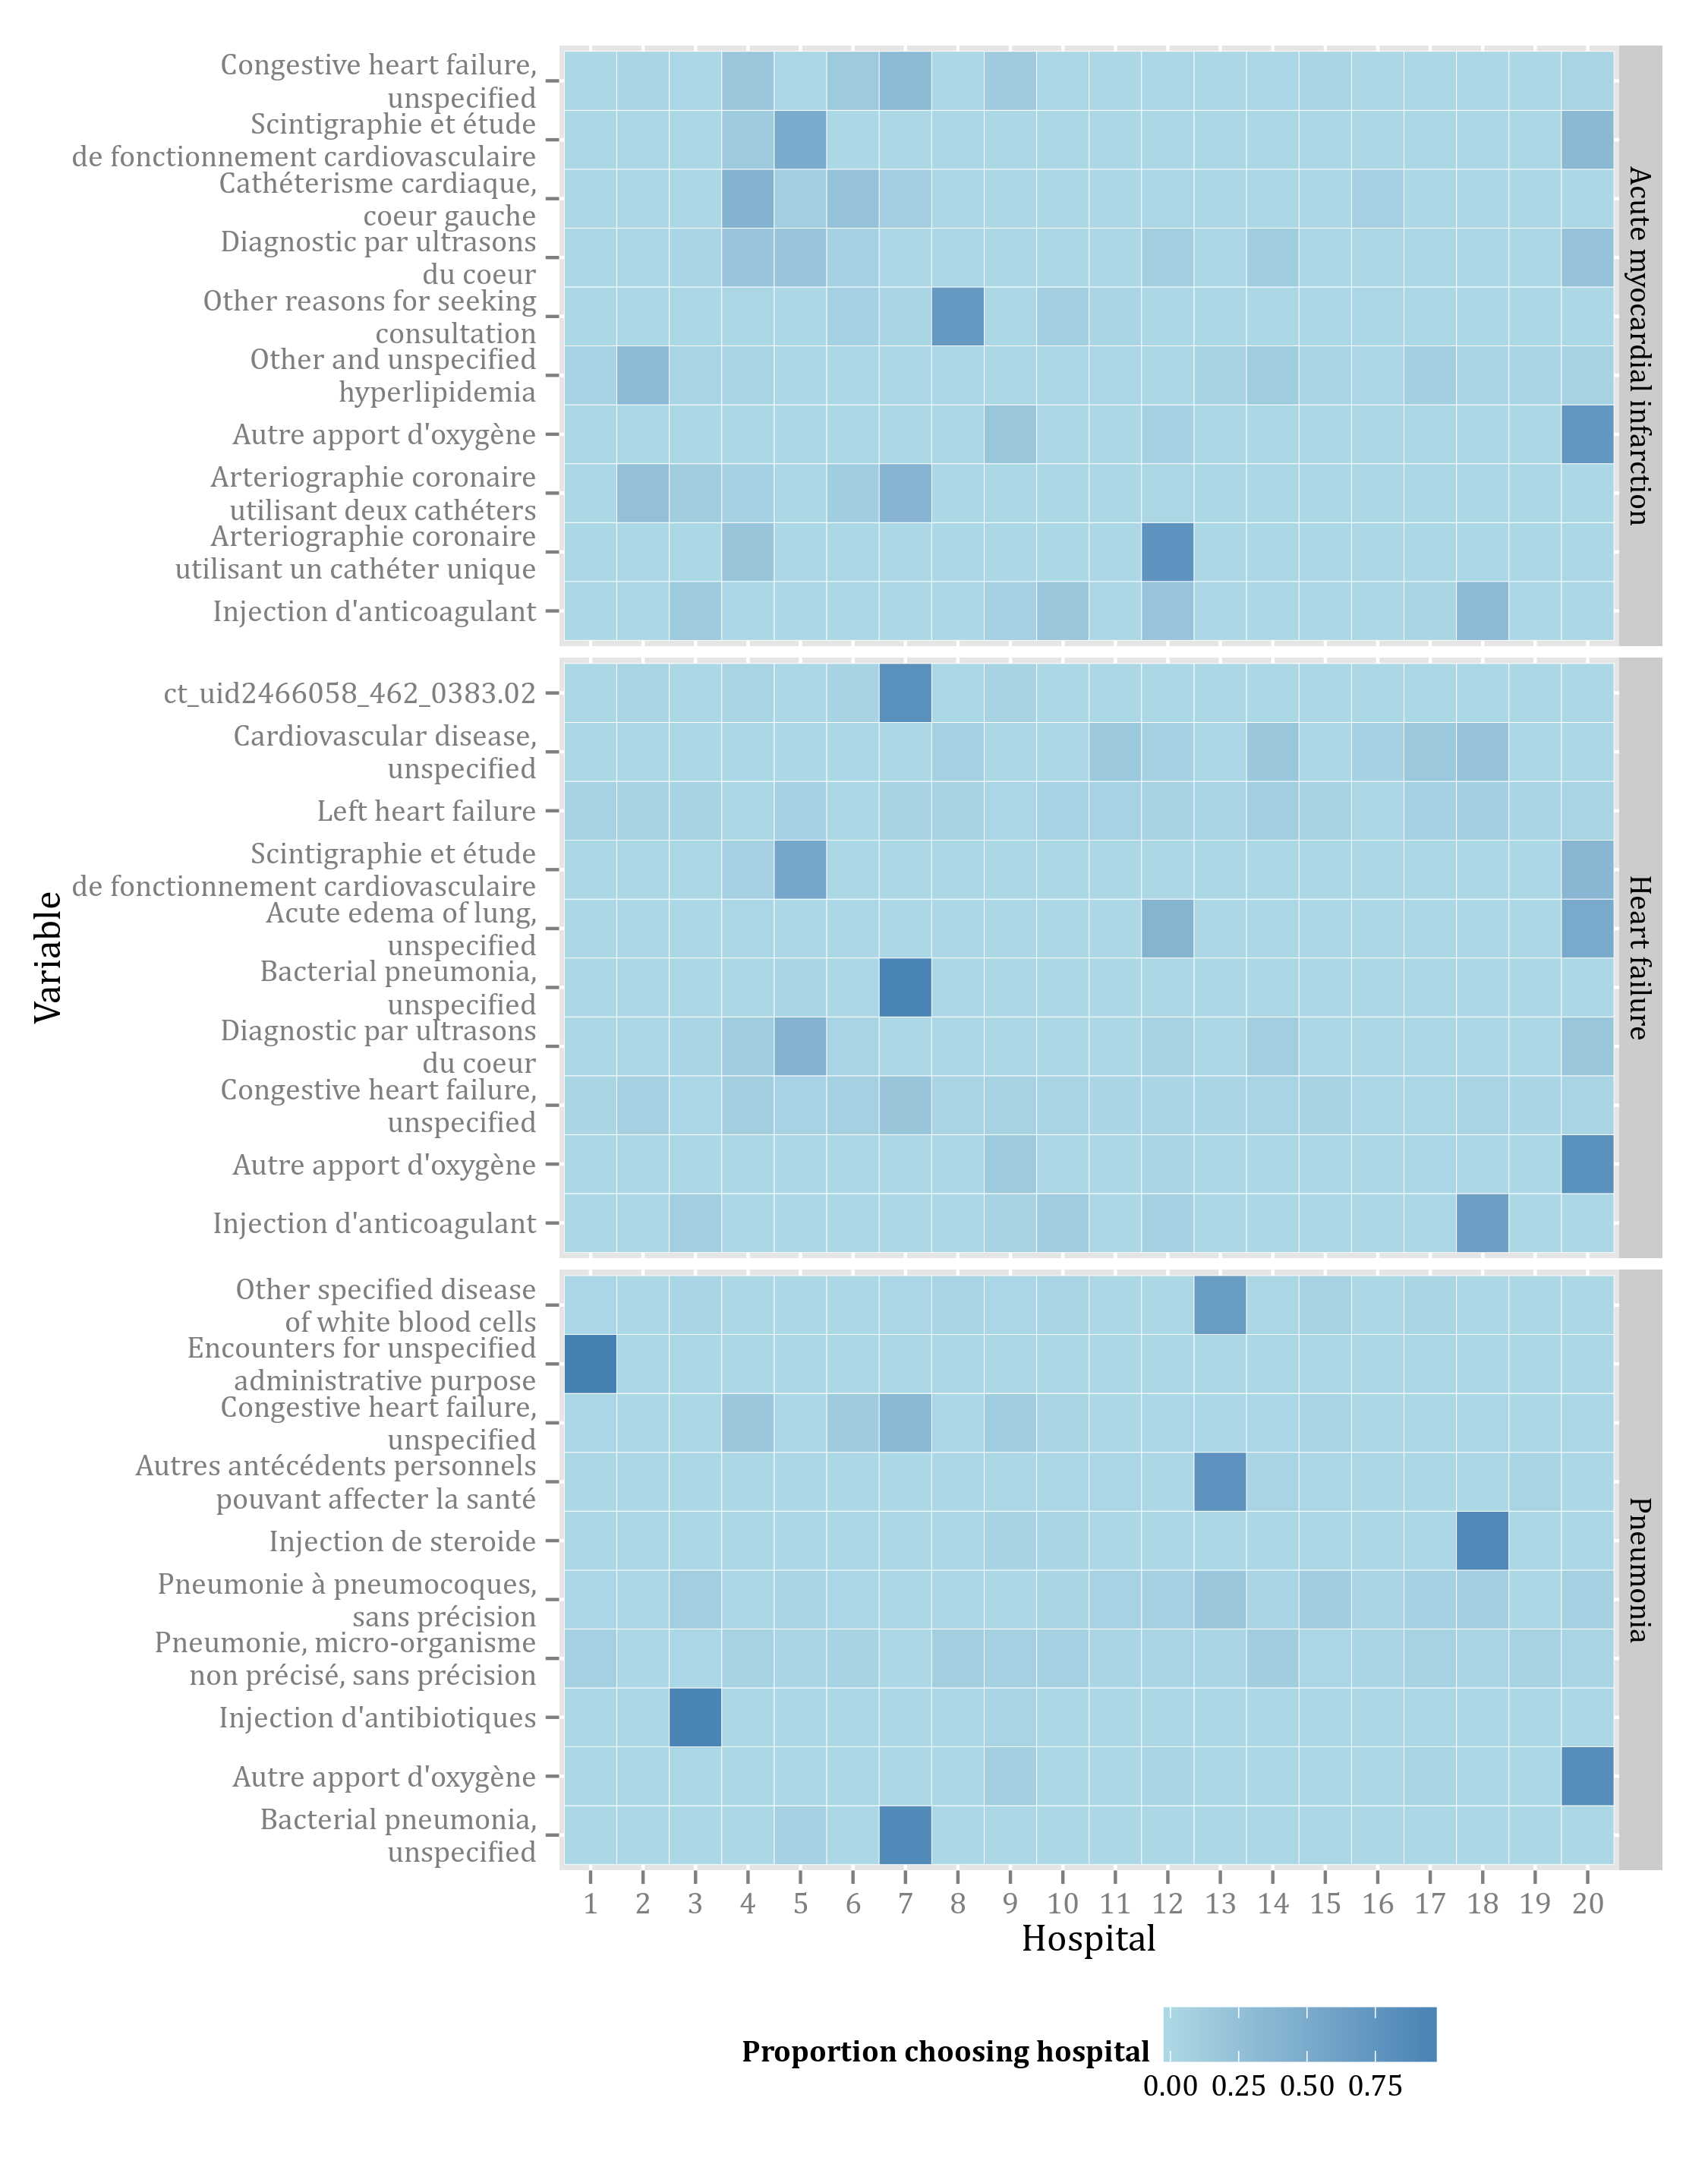
\includegraphics{../figures/top_10_variable_importance_and_hospital.png}
    \caption[Error rate for random forest model of hospital choice.]
      {10 most important variables for the G model, by disease. A descriptive sentence.}
    \label{fig:top_10_variable_importance_and_hospital}
\end{figure}

% How important are the different variables for each model by class?
\begin{figure}[H]
    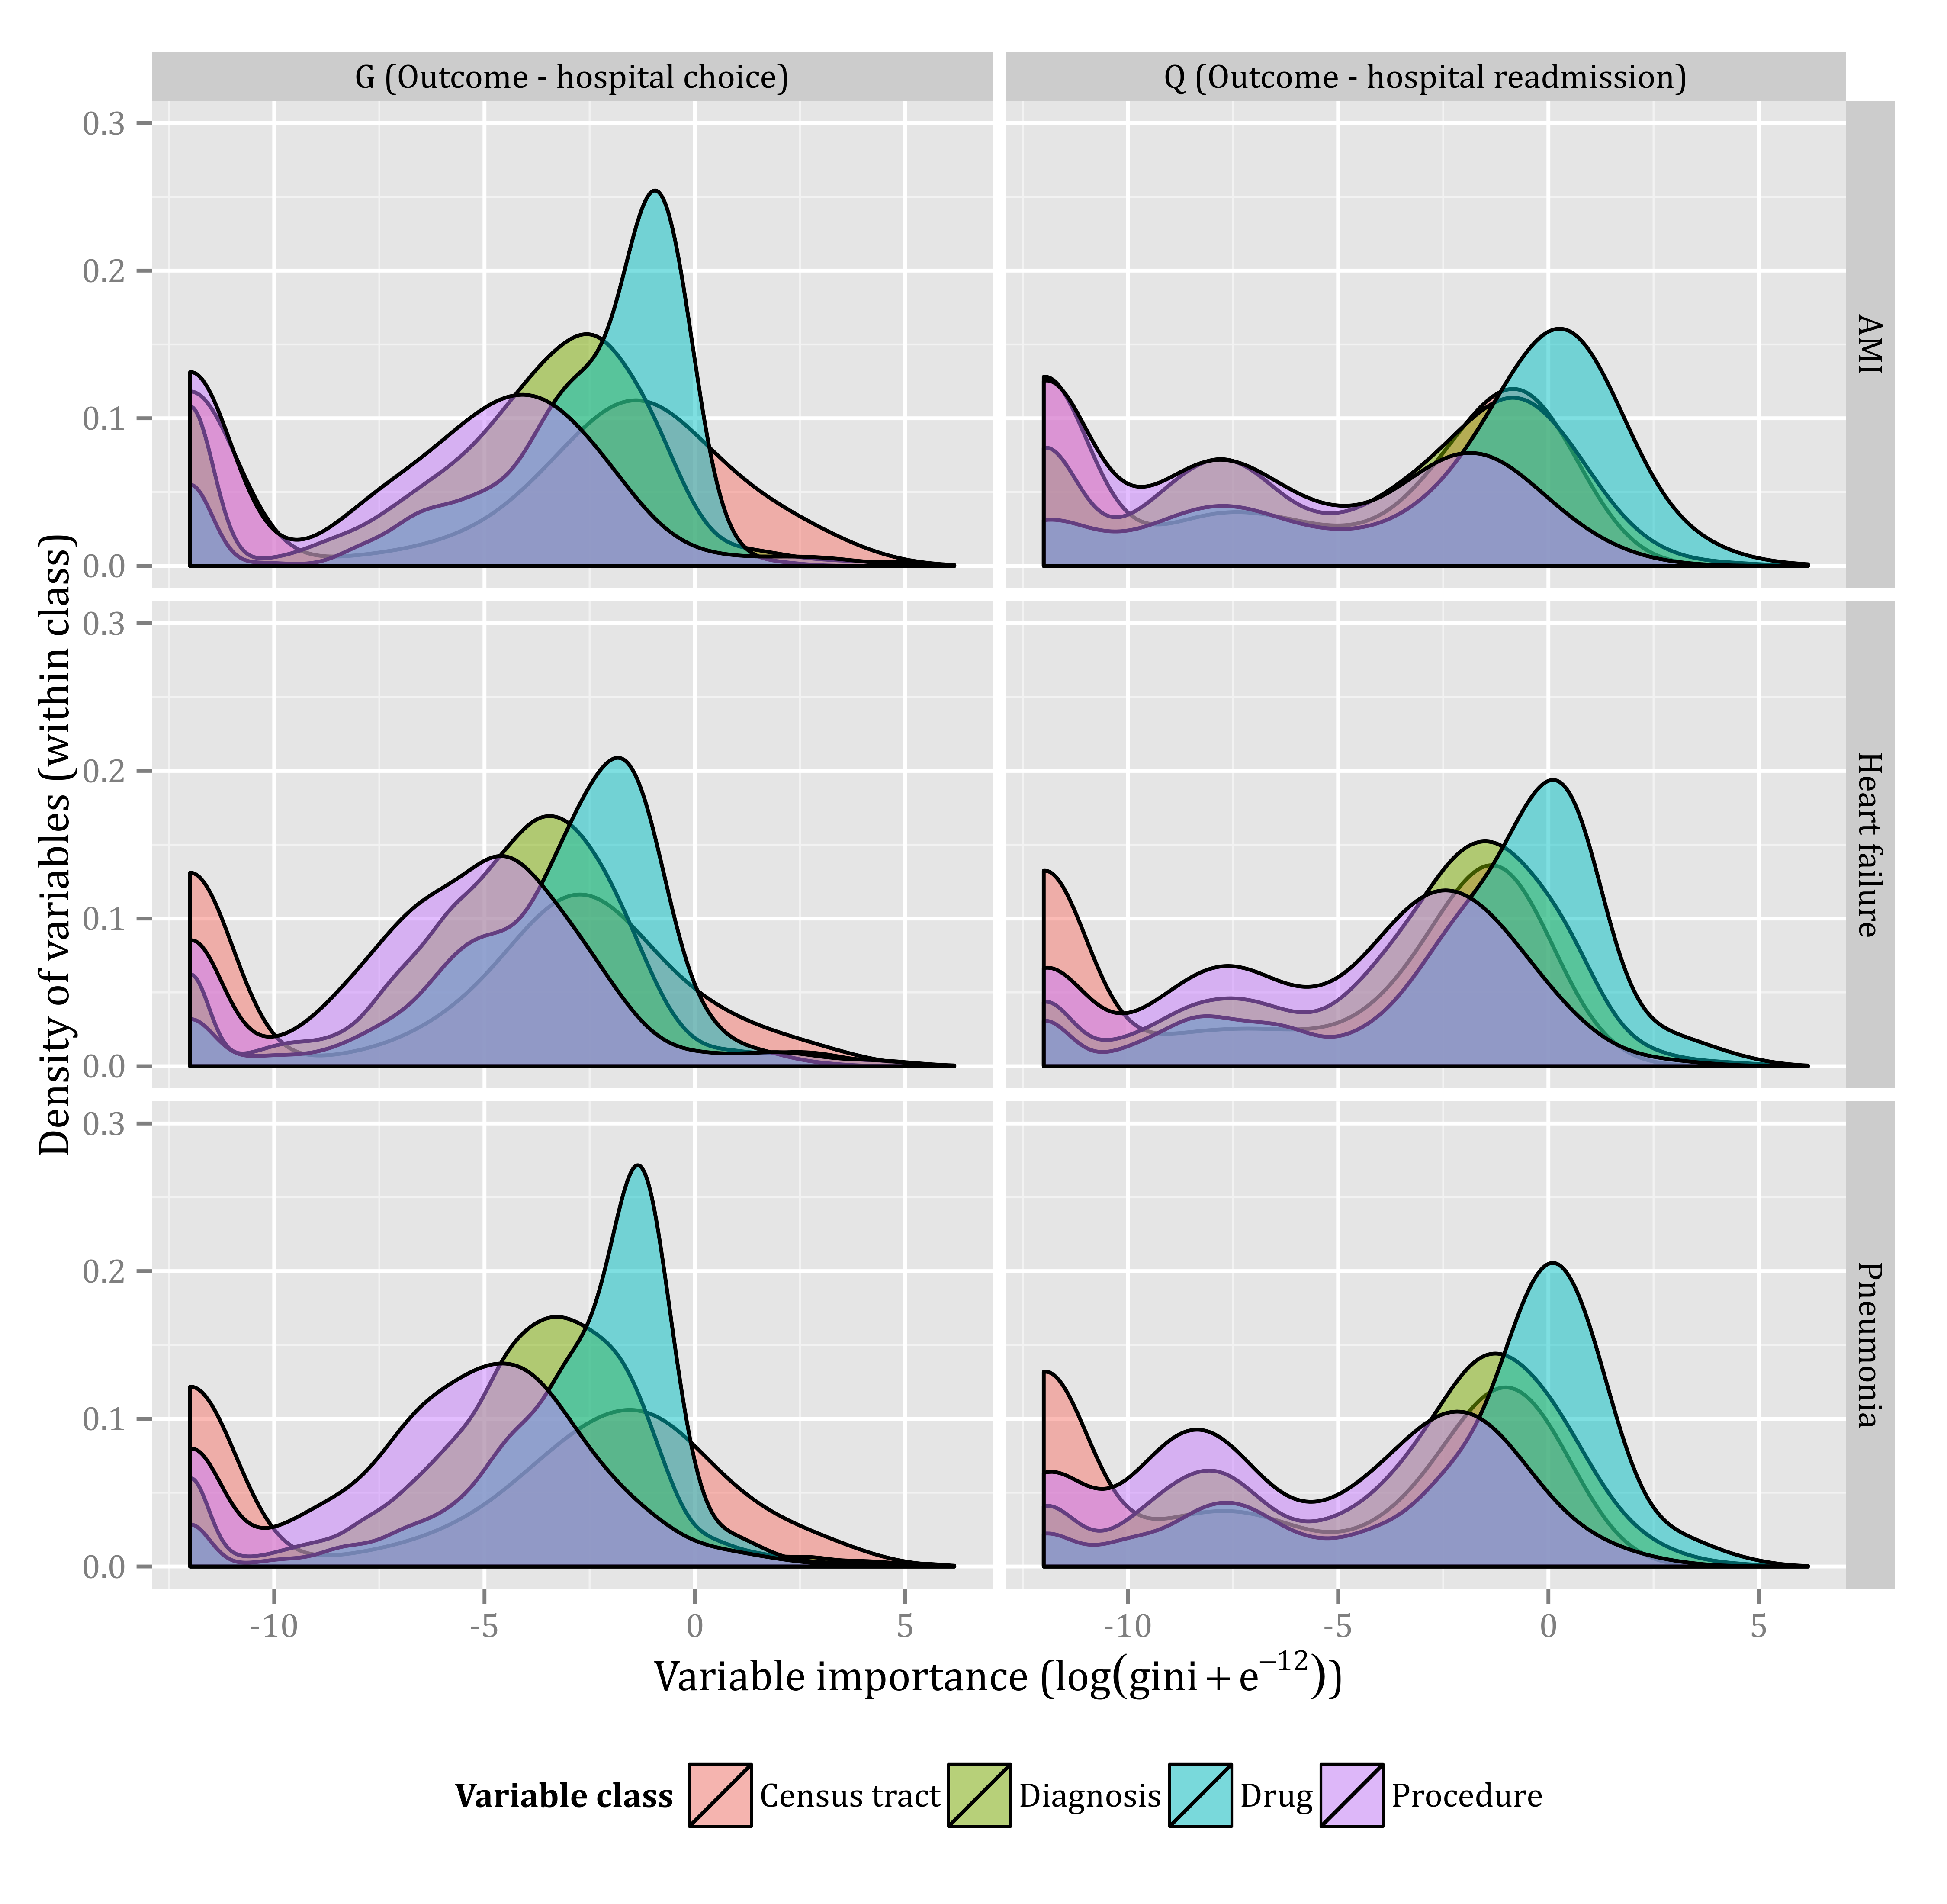
\includegraphics{../figures/variable_importance_by_model_and_class.png}
    \caption[Error rate for random forest model of hospital choice.]
      {Variable importance by model and variable class. A descriptive sentence.}
    \label{fig:variable_importance_by_model_and_class}
\end{figure}

% How does the glmnet model compare accuracy to the random forest model?
% What are the most important variables?

\section{Discussion}


\section{References}
\printbibliography

\end{document}
